\chapter{Project Plan}

The project plan provides a rough outline of all sprints, main activities and their respective time-frames. The project plan is represented by a Gantt-chart found in Appendix \textbf{\ref{app:gantt}}. 

The project is divided into nine sprints of about two weeks, and each sprint has a unique Sprint goal. The last sprints are not planned in full detail to give a buffer for unforeseen time and feature creep.

\section{Presentations}
During the project there will be three presentations. Presentation one is in the start phase of the project, presentation two in the middle of the project and presentation three at the end of the project. A short description of what the different presentations will include is given below. \\\\
\begin{figure}[h]
\begin{minipage}[t]{0.5\textwidth}
\textbf{Presentation 1:}
\begin{itemize}
  \item Presentation of team members
  \item Introduction to the project
  \item The method of execution
  \item Describe the process and project model 
  \item Project plan
  \item Requirements specification
  \item Test specification 
\end{itemize}
\end{minipage}
\hfill
\begin{minipage}[t]{0.5\textwidth}
\textbf{Presentation 2:}
\begin{itemize}
  \item The chosen solution
  \item Present the projects progress
  \item Explain testing
  \item Present the plan forward
\end{itemize}
\end{minipage}
\hfill
\end{figure}\\
\\
\textbf{Presentation 3:}
This presentation is divided into two main parts of 20 minutes. \\
The outline for the first part:
\begin{itemize}
  \item Why the product/solution is the best 
  \item Mention the positive sides of the project and product
  \item Compare the product to other similar products 
\end{itemize}
The outline for the second part:
\begin{itemize}
  \item Lessons Learned
  \item Time usage 
  \item The technical details
  \item A conclusion to the project 
\end{itemize} 



\clearpage

\section{Milestones}


The most important events or points in the project time line are listed as milestones. These are tools which represents multiple activities and focuses on the major events that must be completed in order to achieve success. \\

The milestones give an overview of the work to be done, and serves as a base for committing resources. The Gantt-chart on the other hand, gives a detailed overview of all activities in the entire project from start to finish.  The deadlines are set to ensure that tasks are completed at the right time and provides the stakeholders with information on what they can expect of progress in the various stages of the project. See Tab. \ref{tab:milestones}\\
\begin{table}[h]
\begin{center}
\textbf{\Large Milestones}
\end{center}
\caption{Milestones}
\label{tab:milestones}
\begin{tabular}{llc}
\rowcolor{cadetgrey}
\centering \textbf{Milestone:}    &\textbf{Description:} 	 &\textbf{Expected done:} \\ % &\textbf{Main responsibility:}  \\

\rowcolor{gainsboro}
\textbf{Requirements Identification} & Identify requirements and needs & $13.01.17$ \\
\textbf{Project Plan} & Create a project plan, divide activities, & $24.01.17$ \\
                                     & plan organization & \\
\rowcolor{gainsboro}
\textbf{First Prototype} & Create a simple fixed pitch & $14.02.17$ \\\rowcolor{gainsboro}
                         & quadcopter to test & \\\rowcolor{gainsboro}
                         & flight controller & \\
\textbf{Preliminary Design} & Create a preliminary design & $21.02.17$ \\
                            & for fixed and variable pitch & \\\rowcolor{gainsboro}
\textbf{Basic PID controller} & Develop basic PID controller & $21.02.17$ \\\rowcolor{gainsboro}
                                 & For a fixed and & \\\rowcolor{gainsboro}
                                 & variable pitch quadcopter & \\
\textbf{Basic Flight Controller} & Create a basic flight controller & $28.02.17$ \\
                                 & so the quadcopter can elevate, & \\
                                 & land and go left and right & \\\rowcolor{gainsboro}
\textbf{Fixed Pitch Quadcopter} & Create the fixed pitch quadcopter & $13.03.17$ \\\rowcolor{gainsboro}
                                & (no more changes have been planned) & \\
\textbf{Flight Controller FPQ}  & Finish a flight controller for fixed & $28.03.17$ \\
                                & pitch with possibility for autonomous & \\
                                & and agile flying & \\\rowcolor{gainsboro}
\textbf{Variable Pitch Quadcopter}  & Create the variable pitch quadcopter & $28.03.17$ \\\rowcolor{gainsboro}
                                    & (no more changes have been planned) & \\
\textbf{Flight Controller VPQ}  & Finish a flight controller for variable & $28.04.17$ \\
                            & pitch with possibility for autonomous & \\
                            & and agile flying & \\\rowcolor{gainsboro}
\textbf{Compare fixed and variable pitch}  & Test and compare the quad- & $14.05.17$ \\\rowcolor{gainsboro}
                                           & copters to answer the main & \\\rowcolor{gainsboro}
                                           & requirements & 
\end{tabular}                                                               
\end{table}
\\\\

The table on the next page Tab. \ref{tab:milestonesreworked} illustrates the revised milestones. The milestones are mainly the same, some dates have been changed and one milestone is added. The added milestone is radio control for variable pitch quadcopter.

\begin{table}[H]
\begin{center}
\textbf{\Large Milestones - Reworked}
\end{center}
\caption{Milestones - Reworked}
\label{tab:milestonesreworked}
\begin{tabular}{llc}
\rowcolor{cadetgrey}
\centering \textbf{Milestone:}    &\textbf{Description:} 	 &\textbf{Expected done:} \\ % &\textbf{Main responsibility:}  \\

\rowcolor{gainsboro}
\textbf{Requirements Identification} & Identify requirements and needs & $13.01.17$ \\
\textbf{Project Plan} & Create a project plan, divide activities, & $24.01.17$ \\
                                     & plan organization & \\
\rowcolor{gainsboro}
\textbf{First Prototype} & Create a simple fixed pitch & $14.02.17$ \\\rowcolor{gainsboro}
                         & quadcopter to test & \\\rowcolor{gainsboro}
                         & flight controller & \\
\textbf{Preliminary Design} & Create a preliminary design & $21.02.17$ \\
                            & for fixed and variable pitch & \\\rowcolor{gainsboro}
\textbf{Basic PID controller} & Develop basic PID controller & $21.02.17$ \\\rowcolor{gainsboro}
                                 & For a fixed and & \\\rowcolor{gainsboro}
                                 & variable pitch quadcopter & \\
\textbf{Basic Flight Controller} & Create a basic flight controller & $28.02.17$ \\
                                 & so the quadcopter can elevate, & \\
                                 & land and go left and right & \\\rowcolor{gainsboro}
\textbf{Fixed Pitch Quadcopter} & Create the fixed pitch quadcopter & $13.03.17$ \\\rowcolor{gainsboro}
                                & (no more changes have been planned) & \\
\textbf{Variable Pitch Quadcopter}  & Create the variable pitch quadcopter & $11.04.17$ \\
                                    & (no more changes have been planned) & \\\rowcolor{gainsboro}
\textbf{Radio Control VPQ}  & Modify a fixed pitch flight controller & $18.04.17$ \\\rowcolor{gainsboro}
                                & to work with radio control & \\
\textbf{Flight Controller VPQ}  & Finish a flight controller for variable & $09.05.17$ \\
                            & pitch with possibility for autonomous & \\
                            & and agile flying & \\\rowcolor{gainsboro}
\textbf{Compare fixed and variable pitch}  & Test and compare the quad- & $16.05.17$ \\\rowcolor{gainsboro}
                                           & copters to answer the main & \\\rowcolor{gainsboro}
                                           & requirements & 
\end{tabular}                                                               
\end{table}

\section{Activity List}

Milestones are decomposed into necessary activities that must be done in order to complete the milestones. These activities are important to identify in order to get a sufficient estimate on what tasks, resources and time the project will require. Activities are usually given an expected duration and resource use, in terms of manpower, knowledge and budget.\\
\\
Scrum struggles with the long term time-line and the bigger picture for the whole project. Because of this and the fact that the deadline for the project cannot be moved, a detailed project plan is made in addition to Scrum. \\
\\
The process of identifying activities starts with decomposition of larger tasks (such as milestones, epics and backlog items). Activities are identified by asking "What has to be done" in order to achieve the high level goals. \\
\\
A plan for all the sprints in the project have been made and will be used in combination with in-depth task planning before each sprint. Combining Scrum with an overall project plan helps the team to reach the deadlines and still keep the feedback and agility of Scrum. You can find a list of the initial activities that were identified below.\\
\\

\begin{center}
\textbf{\Large Activity Layout} \\
%\caption{Activity Layout 1}
\begin{tabular}{cllll}
\rowcolor{cadetgrey}
\textbf{ID:}    &\textbf{Activity:} 	 &\textbf{Estimated time:}    &\textbf{Start:}  \\ % &\textbf{Main responsibility:}  \\
    
\textbf{1} & \textbf{Start-Up Phase} & \textbf{260h} & $03.01.17$ 
\\\rowcolor{gainsboro}
1.1       & Documentations     &     &  \\
1.2       & Research     &     &  \\\rowcolor{gainsboro}
1.3       & Project Model     &     & \\
1.4       & Project Plan     &     & 
\\\rowcolor{gainsboro}
1.5       & Requirements     &     & \\
1.6       & Test Specification     &     & 
\\\rowcolor{gainsboro}
1.7       & Document Templates     &    & \\
1.8       & Internal Meetings      &    & 
\\\rowcolor{gainsboro}
1.9       & External Meetings      &    & \\
\textbf{2} & \textbf{Presentation 1}     & \textbf{100h}    & $03.01.17$ 
\\\rowcolor{gainsboro}
2.1     & Preliminary Documentation Refinement  &    & \\
2.2     & Presentation Refinement  &    &
\\\rowcolor{gainsboro}
2.3     & Presentation Practice  &    & \\
\textbf{3} & \textbf{Sprint 1}     & \textbf{360h}     & $17.01.17$ 
\\\rowcolor{gainsboro}
3.1     & First Presentation &  & \\
3.2     & Preliminary Flight Simulation &  & 
\\\rowcolor{gainsboro}
3.3     & Communication With Qualisys &  & \\
3.4     & Mechanical Design Study &  & 
\\\rowcolor{gainsboro}
3.5       & Internal Meetings      &    & \\
3.6       & External Meetings      &    & 
\\\rowcolor{gainsboro}
\textbf{4} & \textbf{Sprint 2}     & \textbf{360h}     & $31.01.17$ \\
4.1     & Electrical Analysis &  &  \\\rowcolor{gainsboro}
4.2     & Electrical Layout &  & \\
4.3     & Electrical Construction & & \\ \rowcolor{gainsboro}
4.4     & Flight Controller & & \\
4.5     & Create Web Page & &  
\\\rowcolor{gainsboro}
4.6     & Mechanical Design & & \\
4.7     & Preliminary Construction & & 
\\\rowcolor{gainsboro}
4.8       & Internal Meetings      &    & \\
4.9       & External Meetings      &    & 
\end{tabular}                                                                   
\end{center}
\newpage

\begin{center}
\textbf{\Large Activity Layout}\\
%caption{Activity Layout 2}
\begin{tabular}{cllll}
\rowcolor{cadetgrey}
\textbf{ID:}    &\textbf{Activity:} 	 &\textbf{Estimated time:}    &\textbf{Start:}  \\ % &\textbf{Main responsibility:}  \\
\rowcolor{gainsboro}
\textbf{5} & \textbf{Sprint 3}     & \textbf{360h}     & $14.02.17$ \\
5.1     & Plan Test Procedures &  &  \\\rowcolor{gainsboro}
5.2     & Mechanical Design &  &  \\
5.3     & Preliminary Variable Pitch Design & & 
\\\rowcolor{gainsboro}
5.4     & Flight Testing and Controll &  & \\
5.5       & Internal Meetings      &    & 
\\\rowcolor{gainsboro}
5.6       & External Meetings      &    & \\
\textbf{6} & \textbf{Sprint 4}     & \textbf{360h}     & $28.02.17$ \\
\rowcolor{gainsboro}
6.1     & Mechanical Design Review & & \\
6.2     & Tweak Flight Controller & & 
\\\rowcolor{gainsboro}
6.3       & Internal Meetings      &    & \\
6.4       & External Meetings      &    & 
\\\rowcolor{gainsboro}
\textbf{7} & \textbf{Sprint 5}     & \textbf{360h}     & $14.03.17$ \\
7.1     & Advanced Controll Functionality &  & \\\rowcolor{gainsboro}
7.2       & Internal Meetings      &    & \\
7.3       & External Meetings      &    & 
\\\rowcolor{gainsboro}
\textbf{8} & \textbf{Presentation 2}     & \textbf{100h}     & $28.03.17$ \\
8.1     & Presentation 2 planning &  &  \\\rowcolor{gainsboro}
\textbf{9} & \textbf{Sprint 6}     & \textbf{360h}     & $28.03.17$ \\
9.1     & Finalize Test Procedures &  & 
\\\rowcolor{gainsboro}
9.2     & Tweak Controller System &  & \\
9.3       & Internal Meetings      &    & 
\\\rowcolor{gainsboro}
9.4       & External Meetings      &    & \\
\textbf{10} & \textbf{Sprint 7}     & \textbf{460h}     & $11.04.17$ \\
\rowcolor{gainsboro}
10.1     & Final Flight Controller Adjustment &  & \\
10.2     & Testing and Comparison & & 
\\\rowcolor{gainsboro}
10.3       & Internal Meetings      &    & \\
10.4       & External Meetings      &    & 
\\\rowcolor{gainsboro}
\rowcolor{gainsboro}
\textbf{11} & \textbf{Sprint 8}     & \textbf{460h}    & $25.04.17$ \\
11.1     & Testing and Comparison              &  &  \\\rowcolor{gainsboro}
11.2     & Documentation &  &  \\
11.3     & Testing & &  \\\rowcolor{gainsboro}
11.4       & Internal Meetings      &    & \\
11.5       & External Meetings      &    & 
\\\rowcolor{gainsboro}
\rowcolor{gainsboro}
\textbf{12} & \textbf{Sprint 9}     & \textbf{460h}     & $09.05.17$ \\
12.1     & Testing and Comparison &  &  \\\rowcolor{gainsboro}
12.2     & Documentation Review &  & \\
12.3       & Internal Meetings      &    & 
\\\rowcolor{gainsboro}
12.4       & External Meetings      &    & \\
\textbf{13} & \textbf{Presentation 3}     & \textbf{100h}     & $09.05.17$ \\
\rowcolor{gainsboro}
13.1     & Documentation Review &  & \\
13.2     & Practice & & \\
\rowcolor{gainsboro}
         & \textbf{Total amount of hours estimated:} & \textbf{4200h} & 
         \\\\\\\\\
\end{tabular}                                                               
\end{center}

\begin{comment}
\subsection{Gantt-chart}

To get an overview of the project plan a Gantt-Chart is used. By using a Gantt-Chart the team gets an overview of the project and its associated tasks. The chart also helps to visualize progress and deviations from the project plan. The chart is frequently used in project management, and is closely followed up by the project leader in order to meet the deadline.

The Gantt-chart is provided as a separate document in Appendix \textbf{\ref{app:gantt}} \\

\end{comment}

\begin{comment}
Things that should be in a project plan/ description:

Scope management
Schedule management
Financial management
Quality management
Resource management
Stakeholder management – New from PMBOK 5[citation needed]
Communications management
Project change management
Risk management
\end{comment}


\clearpage

\chapter{Risk Management}
During the start-up phase and throughout the project life cycle, it is important to analyze the risks involved. A plan for all scenarios identified that could endanger and have negative impact on the project has been made. If risks are not planned for they can interrupt progress and may eventually harm the outcome of the entire project. \bigskip

The risk analysis identifies all possible scenarios that can cause problems and determines the probability and severity of these scenarios. By identifying the scenarios one can minimize or eliminate risks. It is important to always reevaluate the risks at every sprint, this is done in order to keep track of current risks or identify new ones while the project changes. \bigskip

\begin{figure}[H]
    \centering
    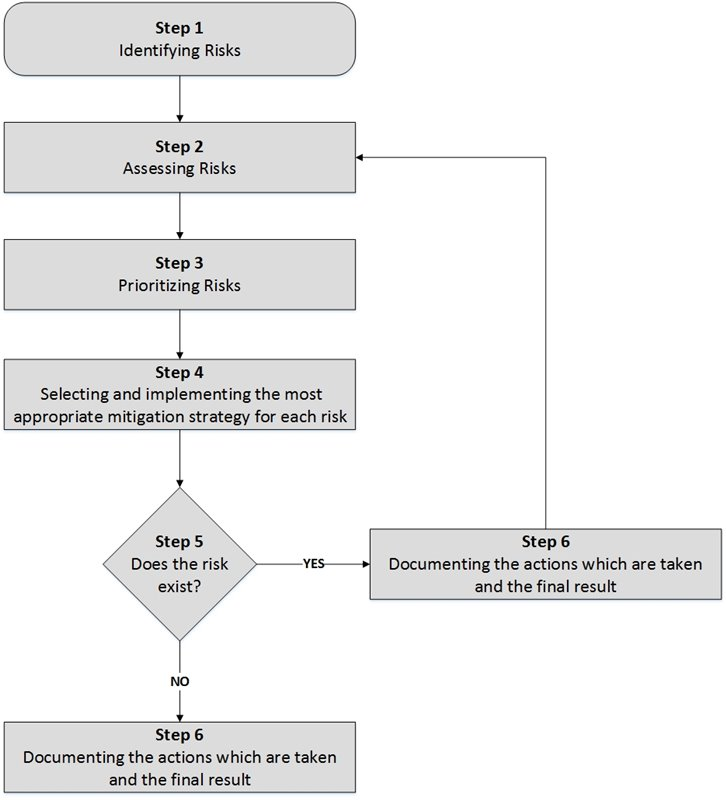
\includegraphics[width = 0.7\textwidth]{VAPIQ-PICTURES/riskprocess.jpg}
    \caption{Risk Identification Process}
    \label{fig:riskid}
\end{figure}
\clearpage
\noindent
Fig. \ref{fig:riskid} shows the risk identification process. Fig. \ref{fig:riskid} are taken from \cite{Alberto}.

\bigskip
Three categories to analyze the risk scenarios are used:
\begin{itemize}
\item{Likelihood of occurrence}
\item{Severity of the scenario}
\item{Detectability (how easy it is to detect the risk)}
\end{itemize}
All risk scenarios are rated according to these three categories with low, medium or high ranking. A likelihood of high, means that the scenario is likely to happen. High severity means that the consequences are severe. High detectability means that it is hard to detect.\bigskip

A risk assessment matrix was developed based on the likelihood of occurrence, severity of the scenario and detectability. This matrix can be seen in Fig. \ref{AssRisk}. The matrix is a helpful tool to visualize risks and how critical they are. A risk is defined as the product between the probability of occurrence times the severity. 

$$Risk = Likelihood\cdot Severity$$ 
\medskip
The Risk assessment matrix is used to determine which Strategy of Action that should be implemented for each risk. 

\begin{figure}[H]
    \centering
    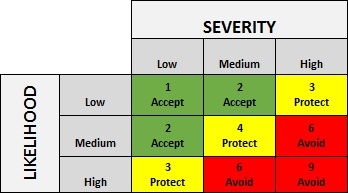
\includegraphics[width = 0.4\textwidth]{VAPIQ-PICTURES/RiskAss.jpg}
    \caption{Risk Assessment Matrix}
    \label{AssRisk}
\end{figure}
\medskip
Three Strategies of Actions (SOA) were developed to handle any risk. Strategies of Actions are any actions that can reduce or eliminate the chance of a risk occurring. Strategies of Action can also be actions that can decrease the severity of the consequences. The Strategies of Actions are:
\begin{itemize}
\item{Accept: Risks with low ranking. No action is needed. No imminent danger.}
\item{Protect: Risks with medium ranking. These risks requires actions to reduce the probability of occurrence.}
\item{Avoid: Risks with high ranking. These risks need to be eliminated or reduced. If the risk occurs, a pre-made plan of action must be in place.}
\end{itemize}\medskip

The Strategies of Acting for Protect and Avoid, are called Mitigation Strategies and are found in Appendix \textbf{\ref{app:riskmatrix}}. \bigskip

Appendix \textbf{\ref{app:riskmatrix}} shows all the different risk scenarios, along with the strategies, likelihood, severity, detectability and origin. Every scenario has its unique Risk ID for traceability.


\begin{comment}
%After analysing all scenarios in the risk assessment matrix, we know that, for instant, sudden new requirements from the customer FFI, can put the project at risk. This is because of limited time and a deadline that is fixed. If this happens we need to adapt and accept it, change the backlog and re-prioritize activities. And since we are using the highly iterative scrum model, it is relatively easy to handle changes. 

%The risk which got the highest rating was wrong estimation of story-points. Estimating wrong will put the whole project in danger in the way that we don't have a product at the end. Most of the highest risks, are connected to requirements. Thus we need to always reevaluate user stories at every sprint review meeting in order to ensure completeness. Budget overrun also is a huge risk. Therefore it is important to do thorough studies before we decide to order parts.

%To ensure low risk it is important to have a risk meeting at the beginning of each sprint. Here we reevaluate the risk scenarios, and analyzes which risks that are most likely to happen during the sprint. During these meetings we must develop plans on how to handle the risks that are most likely to happen.
\end{comment}

\clearpage

\chapter{Budget}
The project budget is 15.000 NOK. The budget will mainly be used to purchase parts and accessories for the quadcopter. A small amount of the budget is used on project management tools, such as Jira and ShareLaTeX.\\

In Fig. \ref{tab:budget} \& \ref{tab:budgetcont} you can see the expenses of the project. In sprint 7, the budget was overran. The overrun was due to ordered parts that turned out to be of bad quality. If all orders had been of the expected quality, the team would still be within the original budget frame. 


\begin{table}[H]
\begin{center}
\textbf{\Large Budget}
\end{center}
\caption{Project Budget }
\label{tab:budget}
\begin{tabular}{|l|l|c|c|}
\rowcolor{cadetgrey}
\centering \textbf{Date:}    &\textbf{Description:} 	 &\textbf{Quantity:} & \textbf{Amount (NOK): } \\ % &\textbf{Main responsibility:}  \\
\hline
\rowcolor{gainsboro} & \textbf{Parts and Components} & & \\ 
                        17.01.2017 & C20 Brushless Outrunner 2050KV  & 4  & 327,45 \\ 
\rowcolor{gainsboro}    17.01.2017 & 4D Hollow Variable Pitch Unit, 3mm Motor Shaft & 4 & 905,69 \\
                        17.01.2017 & Turnigy Multistar 32 bit 12A Race Spec ESC 2~4S & 4 & 367,85 \\
\rowcolor{gainsboro}    17.01.2017 & Towerpro MG90D Mini Digital Servo 2.4kg/0.08sec/13kg & 4  & 156,76   \\
                        17.01.2017 & 7" Variable Pitch Propeller Blades 3D  & 5  & 182,88 \\
\rowcolor{gainsboro}    17.01.2017 & GWS EP Propeller (DD-7035 178x89mm) Black (6pcs/set)  & 2  & 67,06   \\
                        01.02.2017 & HK-500GT Metal Tail Holder Assembly (H50073-H50119)  & 1  & 229,44 \\
\rowcolor{gainsboro}    15.02.2017 & H50054T - Ball Link  & 2  & 52,00   \\
                        15.02.2017 & H50167T 500PRO Linkage Ball Assembly  & 2  & 176 \\
\rowcolor{gainsboro}    15.02.2017 & H50174T 500PRO Linkage Rod Set  & 2  & 92,00  \\
                        15.02.2017 & HD123AT 120 Main blades for T-Rex 150  & 2  & 188,00 \\
\rowcolor{gainsboro}    16.02.2017 & HK-500GT Metal Tail Holder Assembly (H50073-H50119)   & 4 & 425,50   \\
                        16.02.2017 & HK600GT Tail Blade (H60051)  & 4  & 24,03 \\
\rowcolor{gainsboro}    16.02.2017 & Assault 700 DFC - Tail Blades (1 pair)  & 4  & 48,40   \\
                        21.02.2017 & Karbonrør 16x14x1000mm - Bronto   & 1  & 275,00 \\
\rowcolor{gainsboro}    01.03.2017 & Brushless Motor + 4D Metal Variable Pitch + 7" props & 4  & 1659,62  \\
                        19.03.2017 & Batteries, Balancing cable and Lipo BEC regulator & 1 & 751,00 \\
\rowcolor{gainsboro}    19.03.2017 & AXI 2208/26 EVP x2 EVP prop set x8 & 1  & 2500,00   \\
                        20.03.2017 & AXI 2208/26 EVP  & 2 & 682,00 \\
\rowcolor{gainsboro}    21.03.2017 & 9250 IMU Sensor & 4 & 514,00  \\
                        07.04.2017 & Align DS455M Digital Servo 2.9kg/0.04s  & 4 & 1435,00 \\
\rowcolor{gainsboro}    19.04.2017 & EVP Bearing Holder & 1 & 15,00   \\
                        19.04.2017 & Controllable Pitch Propeller 91mm & 1 & 170,00 \\
\rowcolor{gainsboro}    20.04.2017 & Lipo Regulator  & 1 & 225,00    \\
\hline
\end{tabular}                                                               
\end{table}


\begin{table}[H]
\begin{center}
\textbf{\Large Budget - Continuation}
\end{center}
\caption{Project Budget - Continuation }
\label{tab:budgetcont}
\begin{tabular}{|l|l|c|c|}
\rowcolor{cadetgrey}
\centering \textbf{Date:}    &\textbf{Description:} 	 &\textbf{Quantity:} & \textbf{Amount (NOK): } \\ % &\textbf{Main responsibility:}  \\
\hline
\rowcolor{gainsboro} & \textbf{Supplies} & & \\ 
                        23.01.2017 & Colored sheets & 50 & 136,00 \\
\rowcolor{gainsboro}    24.01.2017 & Display book for 1. presentation & 1 & 99,00  \\
                        25.01.2017 & Printer paper  & 1 & 92,00 \\
\rowcolor{gainsboro}    31.01.2017 & Spacers & 1 & 153,00   \\
                        09.02.2017 & Plexiglass 600x600x4mm & 1 & 169,00 \\
\rowcolor{gainsboro}    09.02.2017 & Supplies for test rig & 1 & 349,00   \\
                        01.03.2017 & Supplies for 2 axis test rig  & 1 & 333,50 \\
\rowcolor{gainsboro}    01.03.2017 & Supplies for 2 axis test rig  & 1 & 248,80  \\
                        27.03.2017 & Binder for 2. pres  & 2 & 70,00 \\
\rowcolor{gainsboro}    &  &  &   \\
                        & \textbf{Shipping and Customs} &  & \\
\rowcolor{gainsboro}    17.01.2017 & HobbyKing Order Nr. 1 & 1 & 246,19  \\
                        31.01.2017 & Customs Order Nr. 1 & 1 & 698,00\\
\rowcolor{gainsboro}    15.02.2017 & Shipping from Elefun & 1 & 74,00  \\
                        16.02.2017 & Shipping from HobbyKing Order 16.02.17 & 1 & 156,27 \\
\rowcolor{gainsboro}    09.03.2017 & Customs Order 16.02.17 & 1 & 322,00  \\
                        14.03.2017 & Customs Order 01.03.17 & 1 & 253,00 \\
\rowcolor{gainsboro}    05.04.2017 & Customs Order 21.03.17 & 1 & 291,00  \\
                        20.03.2017 & Shipping from Steve Webb Model Motors (AXI) & 1  & 275,00 \\
\rowcolor{gainsboro}    19.04.2017 & Shipping rom Model Sports Czech Republic  & 1 & 90,00  \\
                        &  &  & \\
\rowcolor{gainsboro}    &  \textbf{\large Sum} &  & \textbf{\large  15437,24}   \\
\hline
\end{tabular}                                                               
\end{table}





% \begin{figure}[H]
%     \centering
%     \includegraphics[width = 0.9\textwidth]{VAPIQ-PICTURES/budget1.png}
%     \caption{VAPIQ Budget}
%     \label{fig:budget}
% \end{figure}